
\documentclass[11pt,a4paper]{article}
\usepackage[hyperref]{acl2018}
\usepackage{times}
\usepackage{latexsym}
\usepackage{amsmath}
\usepackage{graphicx}

\usepackage{url}

\aclfinalcopy \title{Modulazione AM}

\author{Luca Di Liello \\
  Universit\`a degli studi di Trento / Professore temporaneo presso IIS Galileo Galilei \\
  {\tt luca.diliello@alumni.unitn.it} \\
  last edit: 23/11/2018 - 23:13
}



\begin{document}
\maketitle
\begin{abstract}
  Introduzione alla modulazione AM con segnali sinusoidali.
 \end{abstract}

\section{Introduzione}

La modulazione AM (Amplitude Modulation) è una delle tecniche classiche per la trasmissione di un segnale analogico. Essa si basa, come indica il nome, sulla modifica dell'ampiezza di un segnale detto portante. La $portante$ avrà quindi un ampiezza che varierà nel corso del tempo in funzione dell'ampiezza di un altro segnale, detto $modulante$. La modulazione AM richiede che la frequenza del segnale portante sia molto maggiore della frequenza del segnale modulante, altrimenti si avrebbero degli effetti indesiderati sulla qualità della trasmissione. 

\section{Modulazione}

Le figura \ref{fig:c_mod} mostra il caso in cui le frequenze della portante e della modulante sono sufficientemente differenti per garantire una corretta modulazione. La figura \ref{fig:w_mod} mostra invece cosa accade nel caso di frequenze troppo simili. 

\begin{figure}
  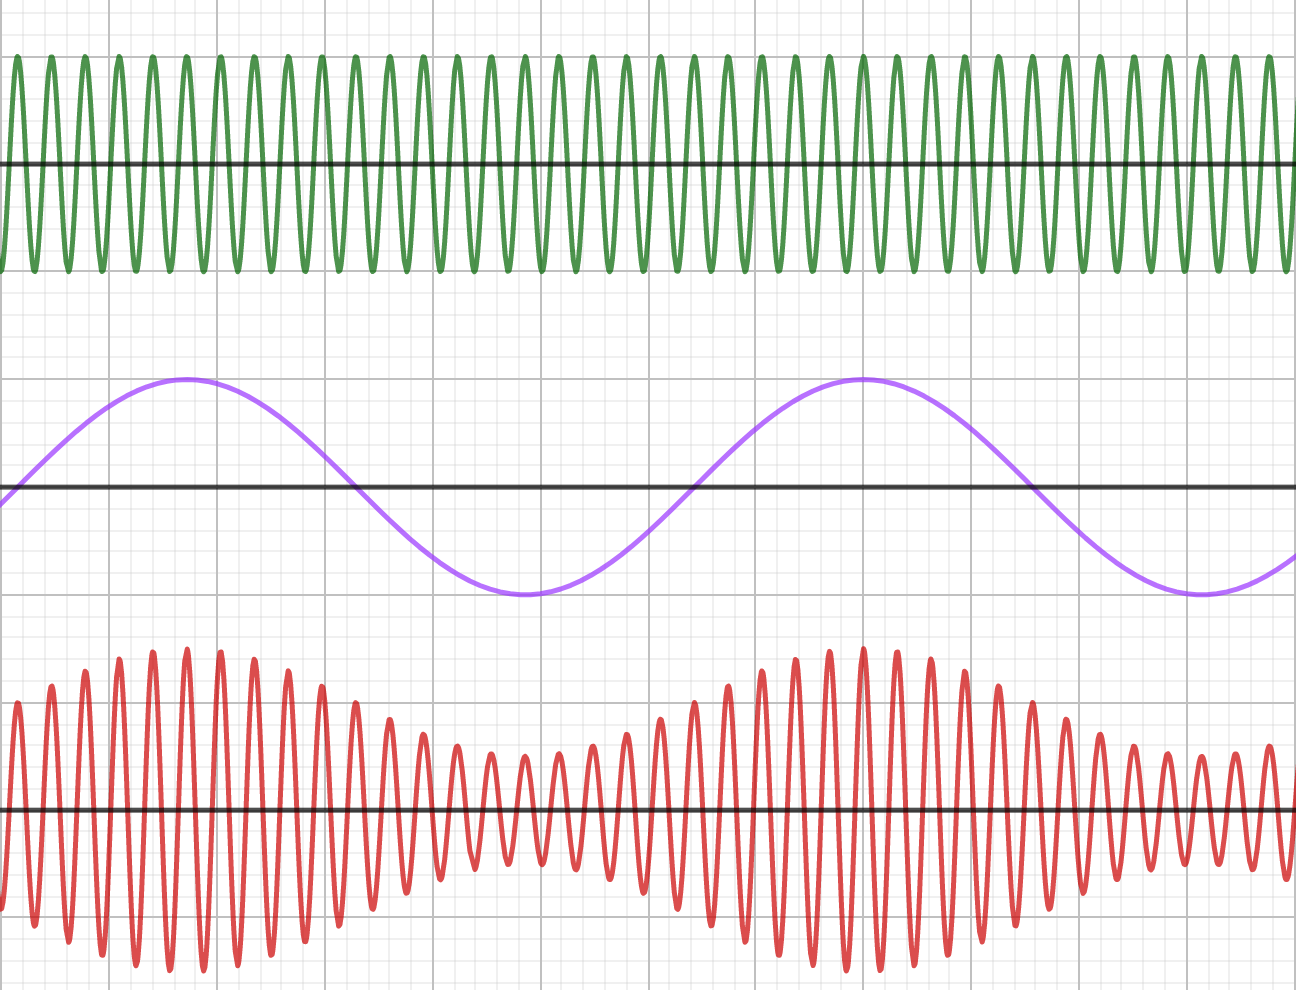
\includegraphics[width=\linewidth]{images/correct_mod.png}
  \caption{$\omega_p >> \omega_m$}
  \label{fig:c_mod}
\end{figure}

\begin{figure}
  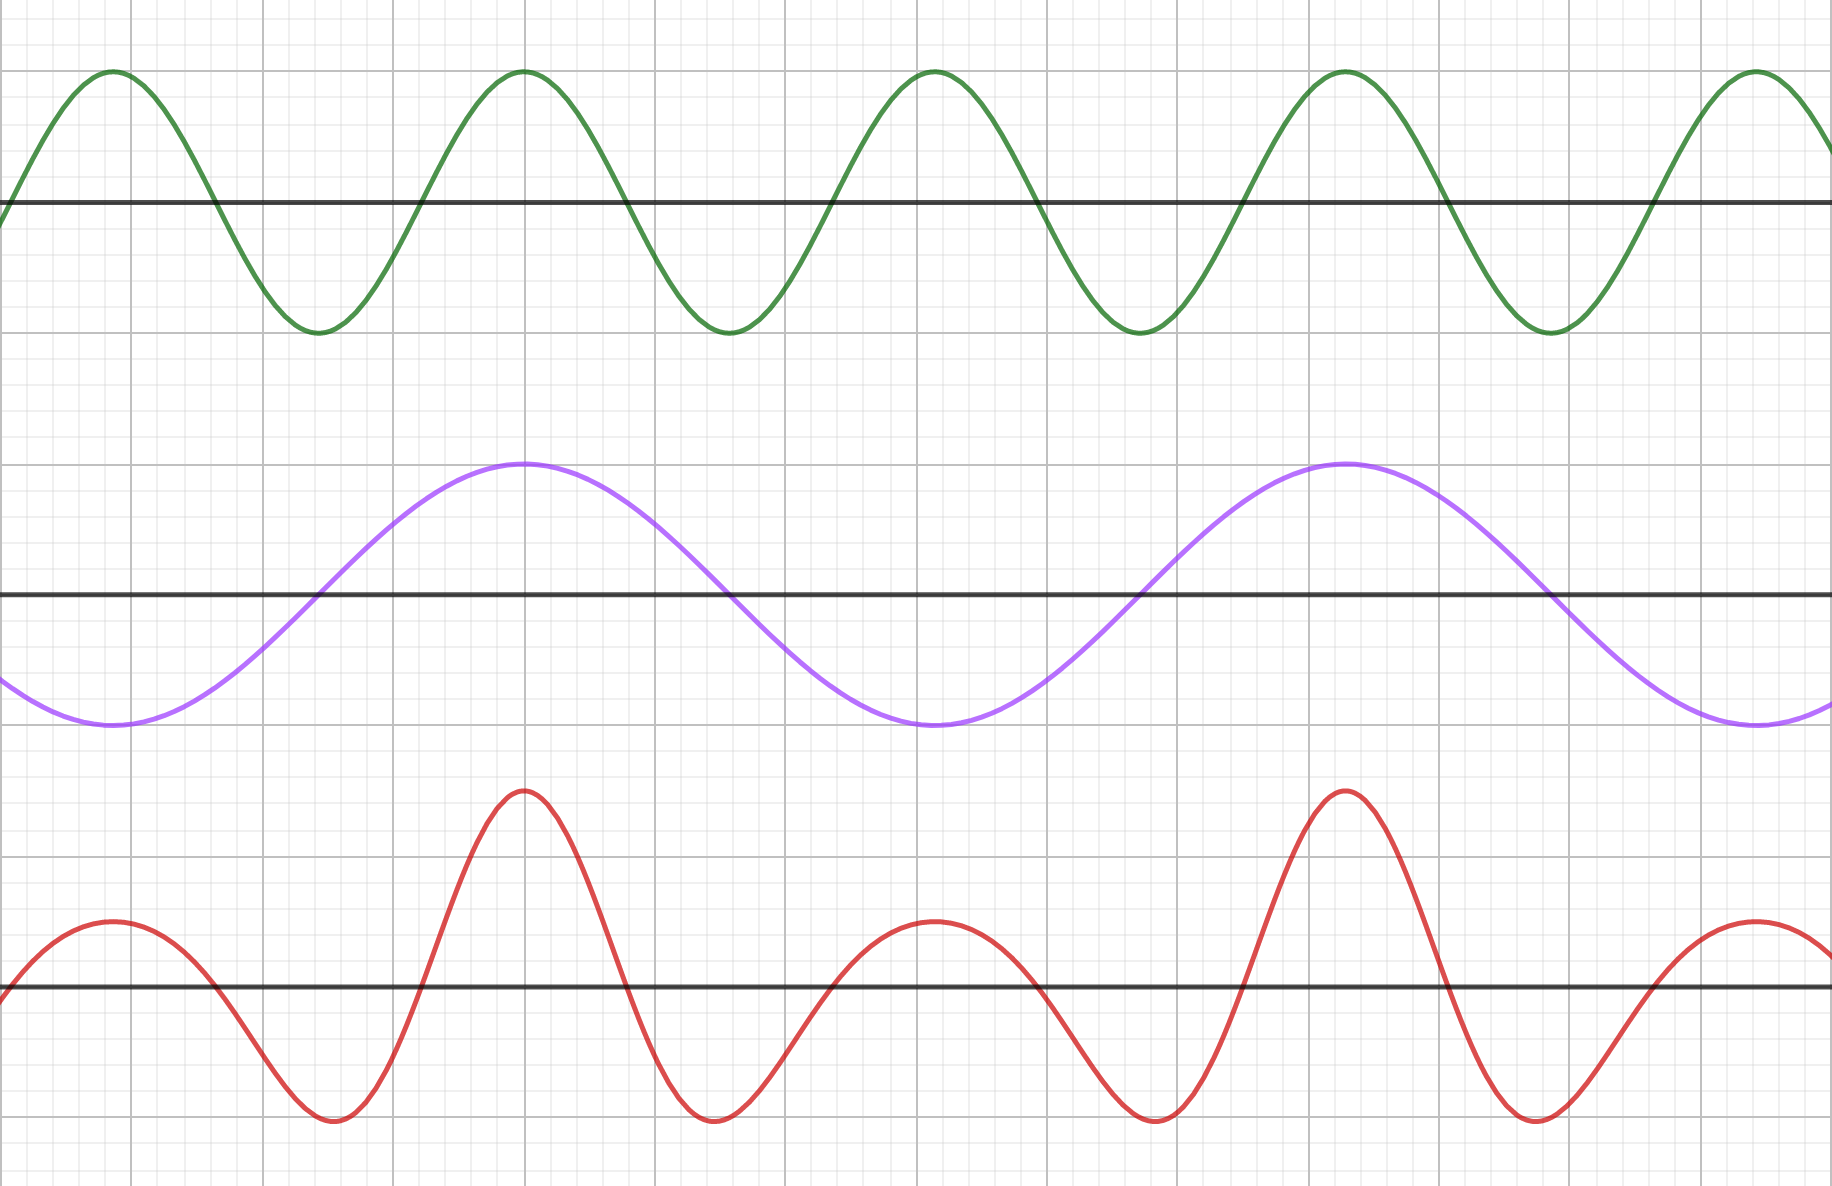
\includegraphics[width=\linewidth]{images/wrong_mod.png}
  \caption{$\omega_p  \approx \omega_m$}
  \label{fig:w_mod}
\end{figure}

In questa semplice trattazione supporremo che il segnale modulante sia anch'esso un segnale sinusoidale, caratterizzato dall'equazione:
$$
m(t) = V_m * cos(\omega_m t + \phi)
$$
Come al solito, la pulsazione angolare sarà pari a:
$$
\omega = 2 \pi F
$$
Dato che non lavoreremo con le fasi, è comodo porre $\phi = 0$. Il segnale portante è molto simile al segnale modulante:
$$
p(t) = V_p * cos(\omega_p t)
$$

Ora la domanda che sorge spontanea è: come unire questi due segnali? La modifica dell'ampiezza del segnale portante non è così semplice come una somma o un prodotto dei segnali! L'equazione seguente mostra come viene creato il segnale modulato:
$$
s(t) = (V_p + K_a * V_m * cos(\omega_m t) ) cos(\omega_p t)
$$
Da questa formula si possono dedurre i passaggi necessari a modulare la portante:
\begin{itemize}
\item Si parte con $p(t)$ e $m(t)$, rispettivamente portante e modulante
\item $m(t)$, che è $V_m * cos(\omega_m t)$, viene moltiplicato per una costante $K_a$
\item $K_a * V_m * cos(\omega_m t)$ viene sommato con $V_p$
\item Infine si moltiplica tutto per $cos(\omega_p t)$
\end{itemize}

I primi 3 passaggi hanno uno scopo ben preciso: il segnale modulante deve essere trasformato in un segnale completamente positivo. Ricordo che il coseno assume valori tra -1 e 1! La figura \ref{fig:using_scaling} mostra come avviene la modulazione se il segnale $m(t)$ viene prima ridotto in ampiezza e poi spostato verso l'alto di $V_p$. La figura \ref{fig:not_using_scaling} mostra invece cosa succede se si esegue direttamente la moltiplicazione dei due segnali senza preoccuparsi dei valori negativi che $m(t)$ può assumere. Perché tutta questa necessità di rendere il modulante completamente positivo? Semplicemente perché le oscillazione del coseno nella parte negativa andrebbero a creare perturbazioni non volute come quelle di figura \ref{fig:not_using_scaling}, dove la "cresta" del segnale risultante non segue più l'andamento del segnale modulato.

\begin{figure}
  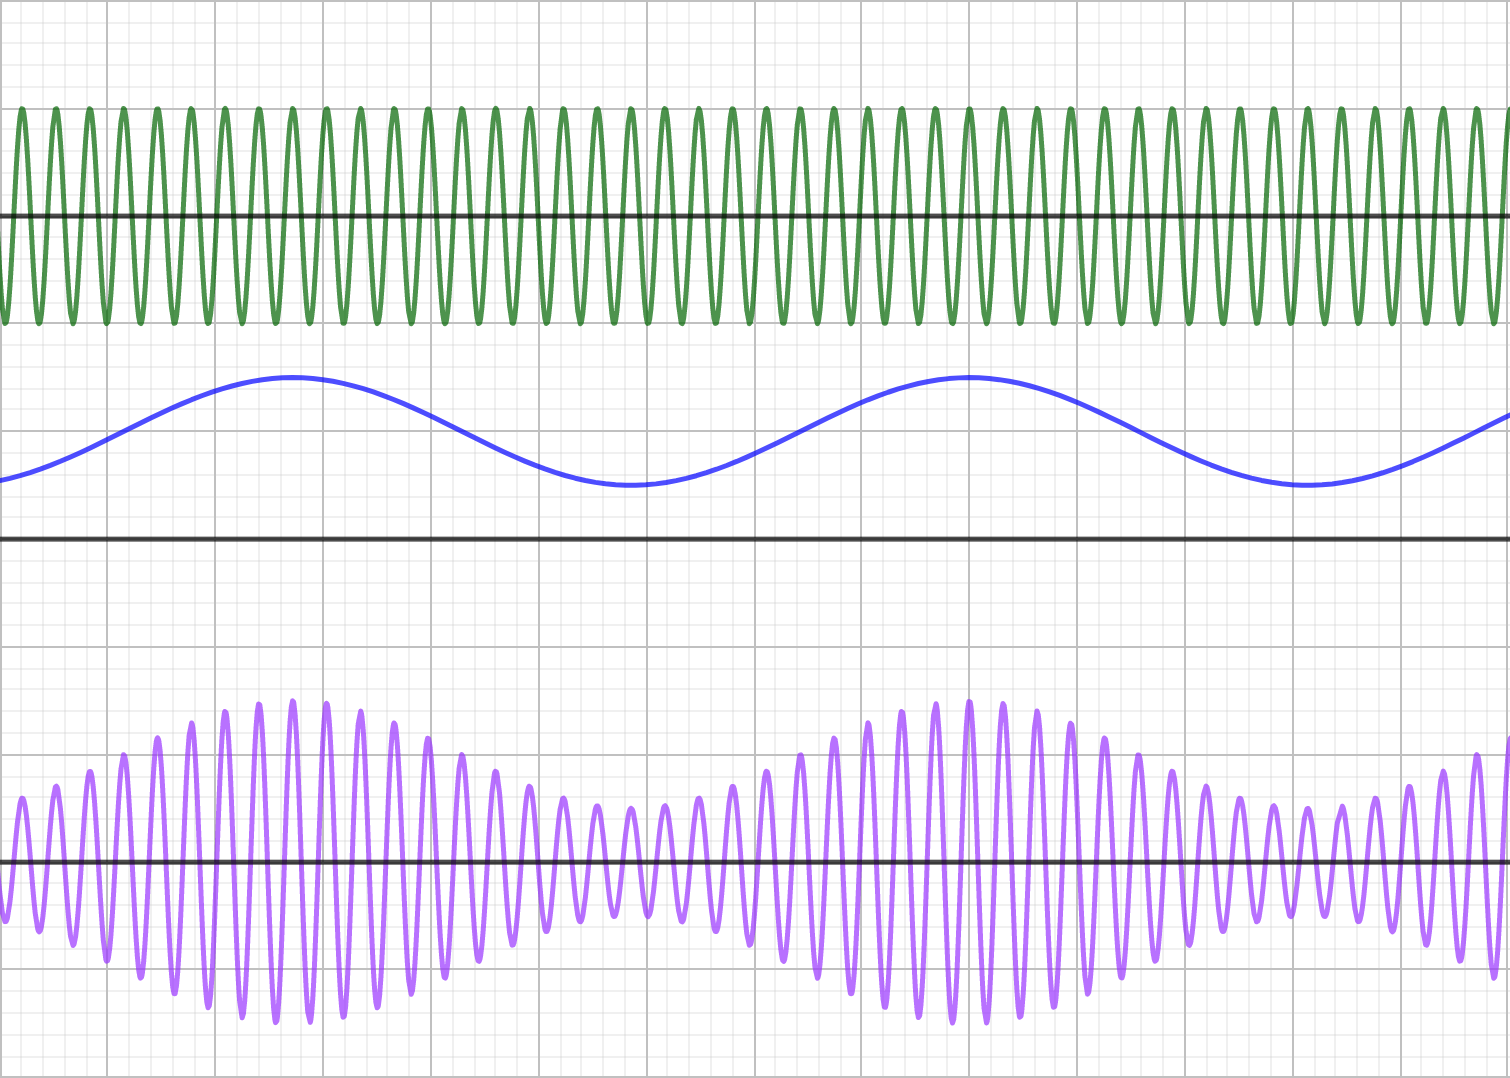
\includegraphics[width=\linewidth]{images/us.png}
  \caption{Modulazione rendendo $m(t)$ sempre positivo}
  \label{fig:using_scaling}
\end{figure}

\begin{figure}
  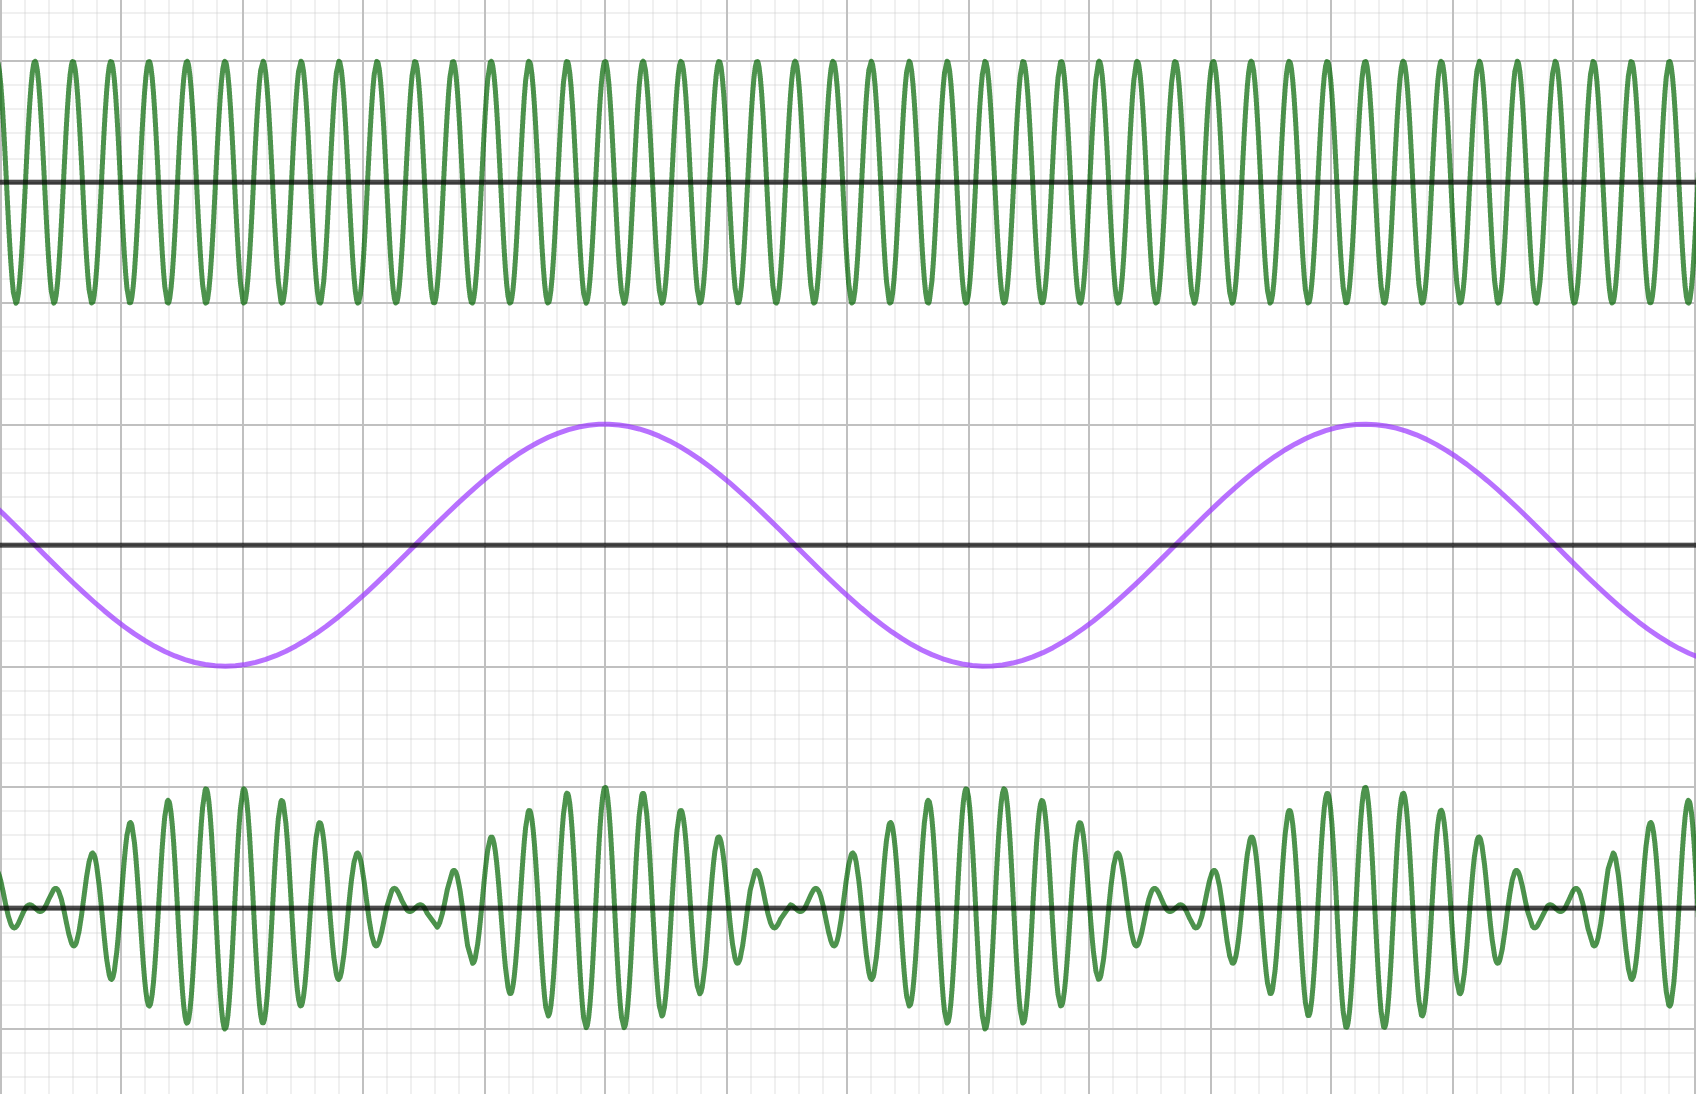
\includegraphics[width=\linewidth]{images/nus.png}
  \caption{Modulazione senza modifica di $m(t)$}
  \label{fig:not_using_scaling}
\end{figure}

\subsection{Parametri della modulazione}

Ritornando al nostro segnale modulato:
$$
s(t) = (V_p + K_a * V_m * cos(\omega_m t) ) cos(\omega_p t)
$$
possiamo raccogliere $V_p$ ed ottenere:
$$
s(t) = V_p (1 + K_a * \frac{V_m}{V_p} * cos(\omega_m t) ) cos(\omega_p t)
$$
Ora, ponendo un nuovo parametro $m_a = K_a * \frac{V_m}{V_p}$, infine otteniamo:
$$
s(t) = V_p (1 + m_a * cos(\omega_m t) ) cos(\omega_p t)
$$
Questo parametro $m_a$ è detto coefficiente di modulazione e deve essere necessariamente:
$$
m_a \leq 1
$$
$m_a$ è chiamato indice di modulazione. La figura \ref{fig:ma} mostra un segnale modulato con diversi valori di $m_a$.

\begin{figure}
  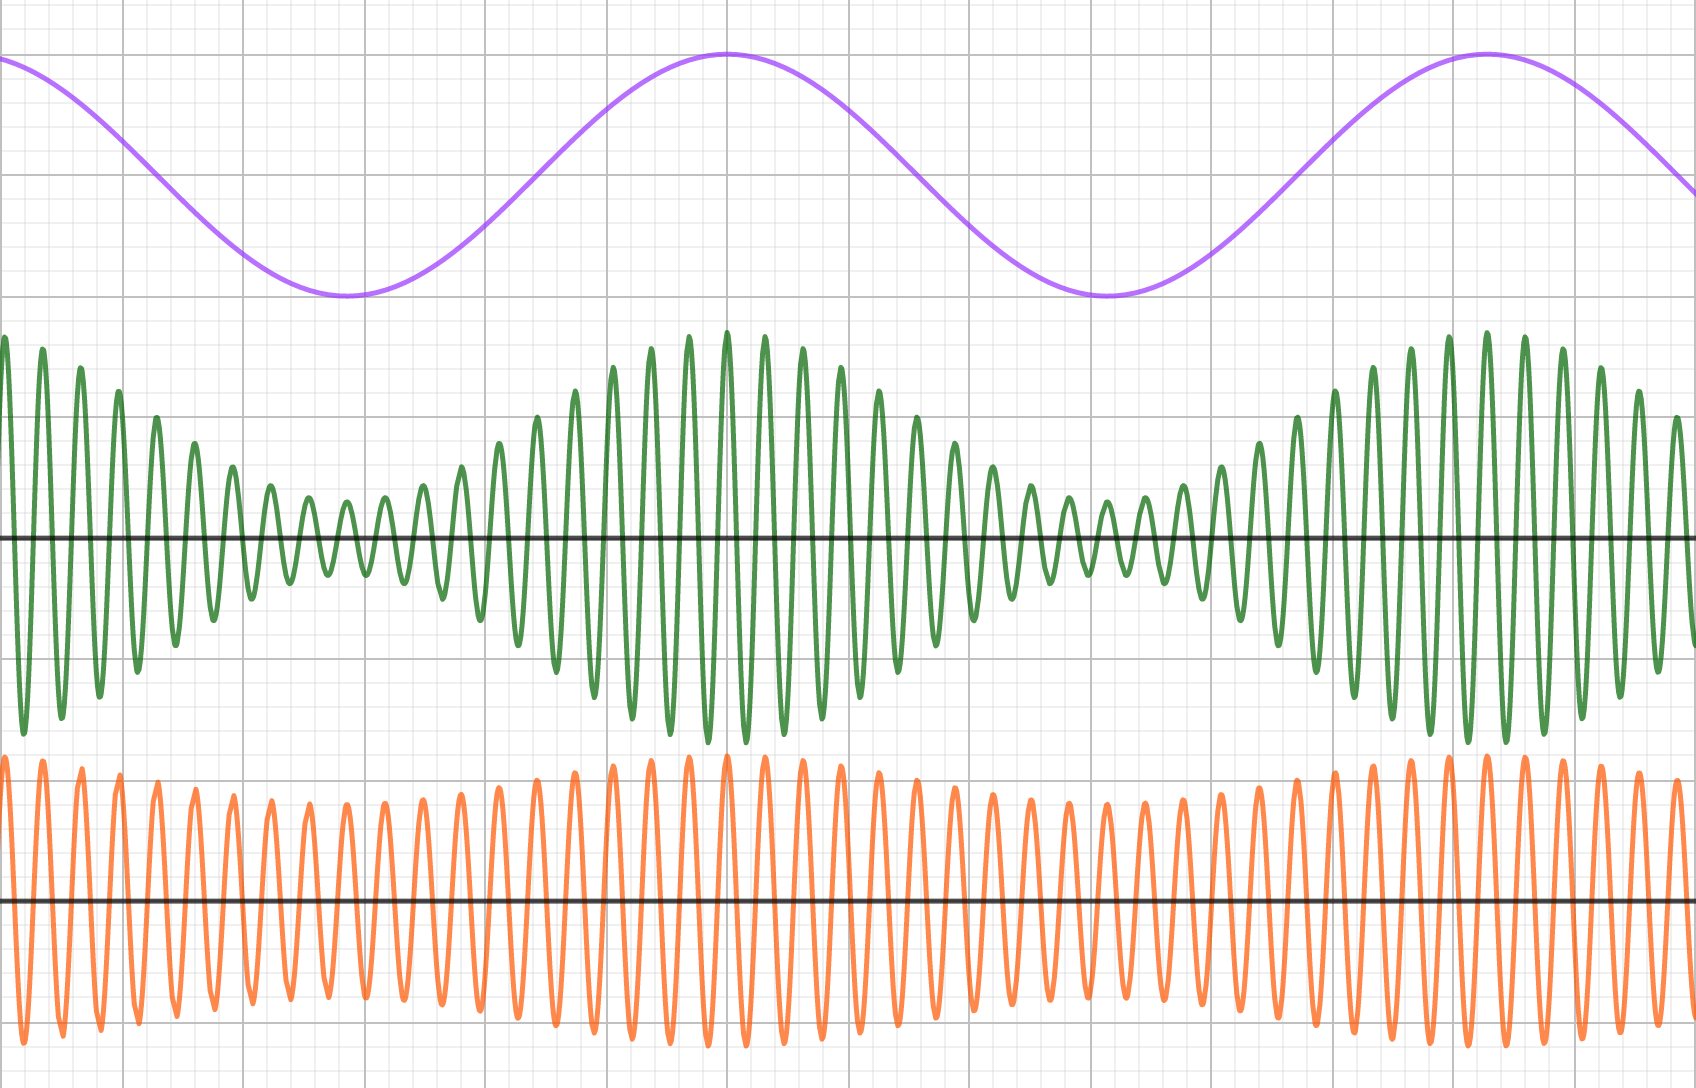
\includegraphics[width=\linewidth]{images/ma.png}
  \caption{$m_a$ grande (sopra) e $m_a$ piccolo (sotto)}
  \label{fig:ma}
\end{figure}

\section{La serie di Fourier}

Spesso in telecomunicazioni, per esigenze di progettazione, è comodo lavorare nel dominio delle frequenze. La serie di Fourier è una funzione matematica che permette di estrarre le componenti sinusoidali che formano un certo segnale $f(t)$. Il grafico tensione-frequenza che si sostituisce a quello solito tensione-tempo, mostra le varie componenti che vanno a formare un certo segnale. Data la complessità della trasformata di Fourier (che richiede la conoscenza degli integrali), verrà trattata solo tramite alcuni semplici esempi.
L'unica formula di cui ci serviremo è quella generale per indicare un segnale come composizione di "armoniche" (sinusoidi) a diversa frequenza. La componente a frequenza più bassa è chiamata $fondamentale$ ed è quella con ampiezza maggiore. Se il segnale è periodico, il numero di componenti è limitato, altrimenti può tendere verso l'infinito. In generale vale la seguente formula, dove $C_k$ sono le ampiezza (complesse) delle componenti: 
$$
f(t) = \sum_{k=1}^{\infty} C_k * \sin(w_k t)
$$
Un buon esempio per capire come le sinusoidi possono comporre un segnale è utilizzare l'onda quadra. L'onda quadra, se analizzata con gli algoritmi di Fourier, risulta essere composta da tutte le armoniche a frequenza dispari $(1,3,5,...)$ con ampiezze man mano decrescenti. La scomposizione dell'onda quadra è:
$$
q(t) = \sum_{f \in \{1,3,5,7,...\}} \frac{1}{f} * \sin(2 \pi f t)
$$
Nella figura \ref{fig:fourier} è mostrata l'approssimazione con man mano sempre più componenti.

\begin{figure}
  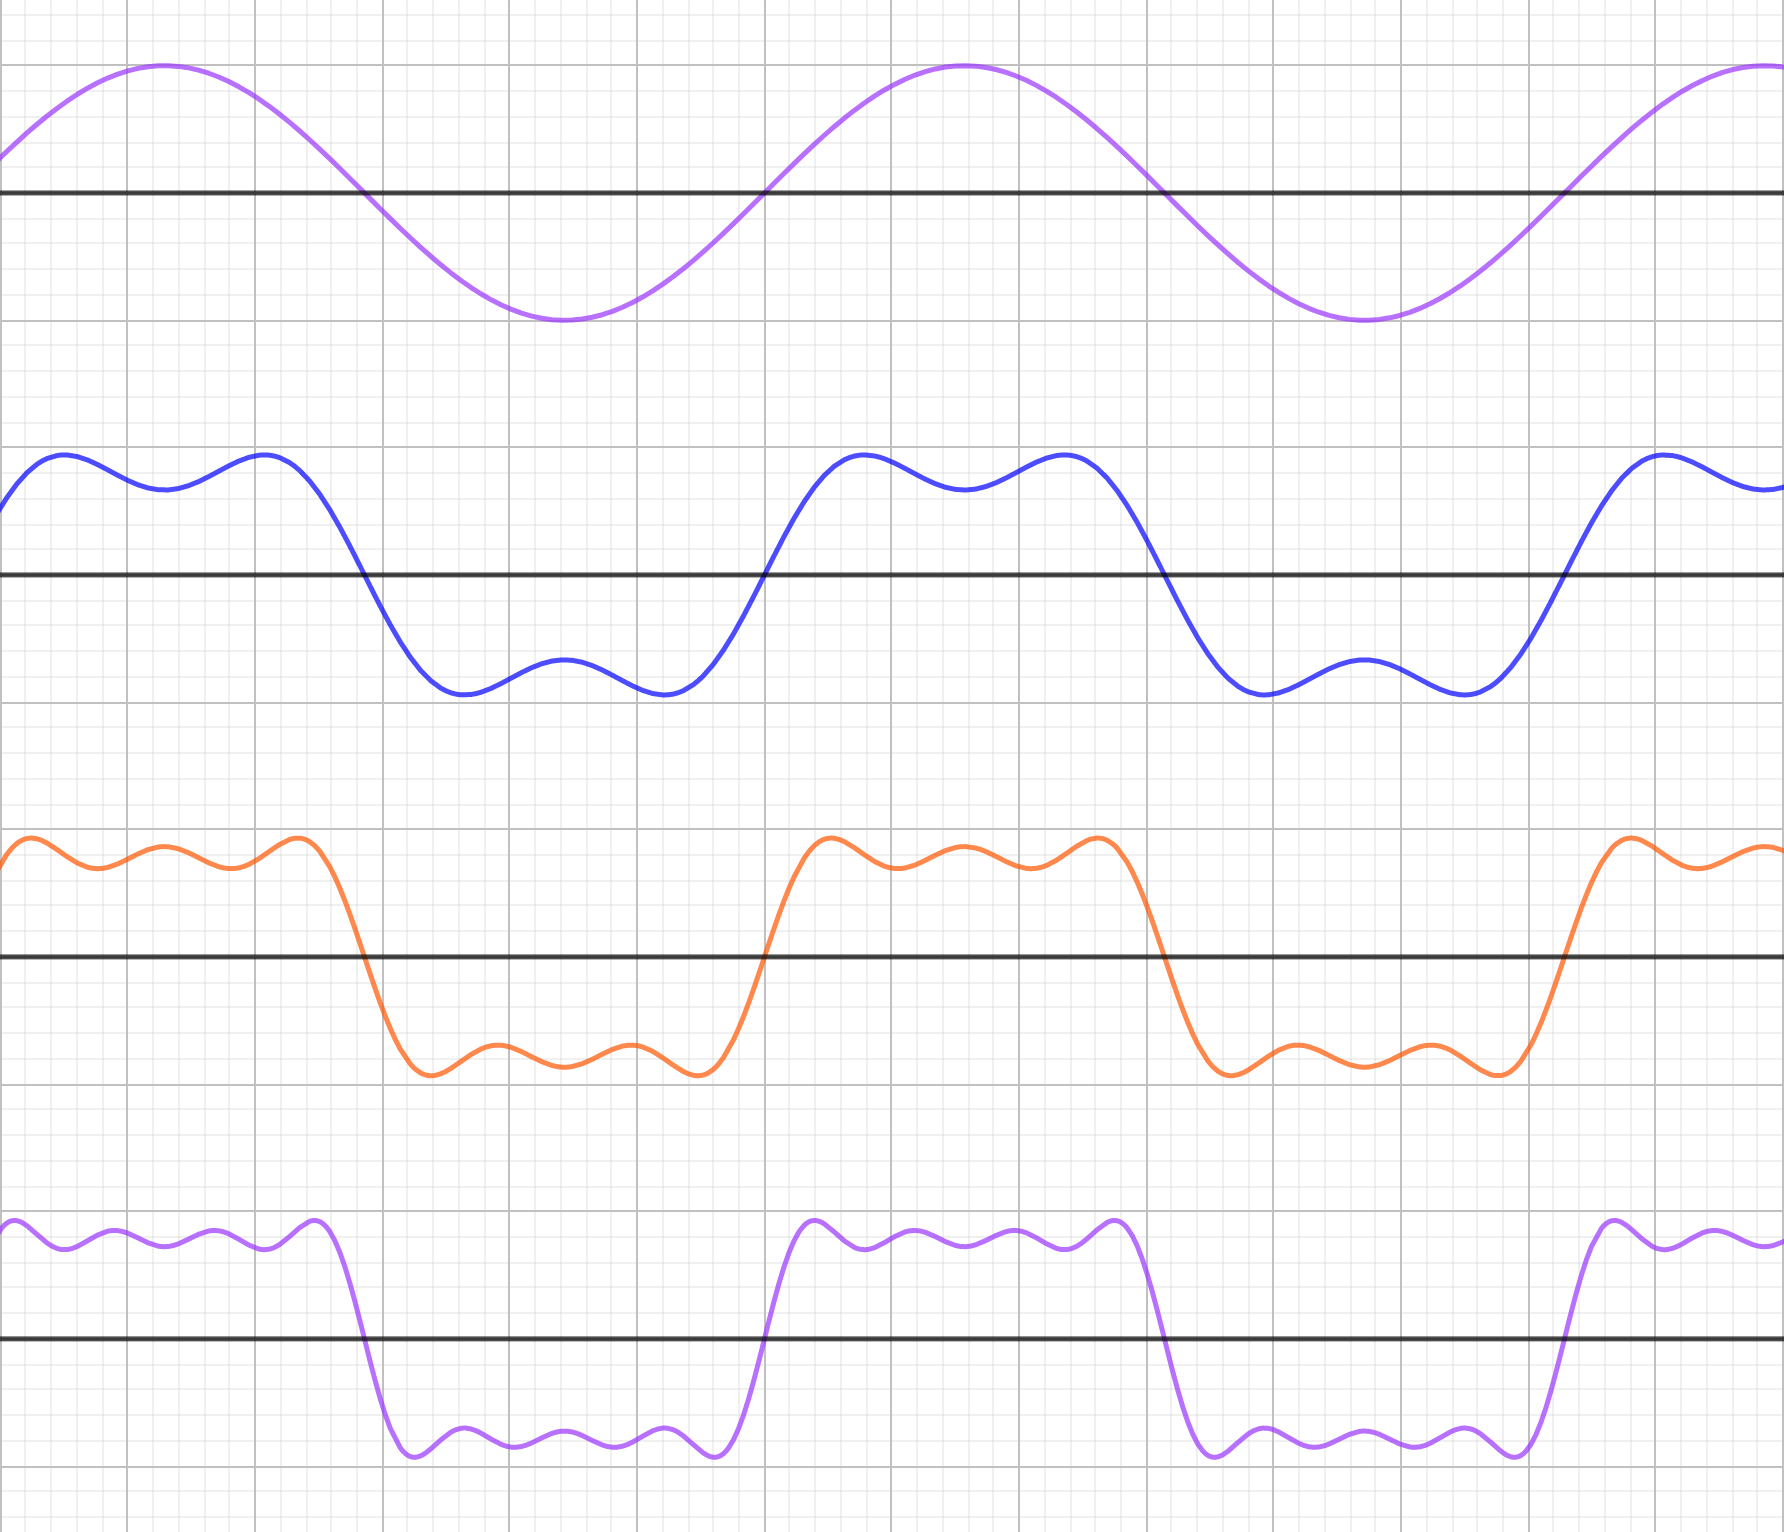
\includegraphics[width=\linewidth]{images/oq.png}
  \caption{Approssimazione dell'onda quadra con 1,3,5,7 armoniche}
  \label{fig:fourier}
\end{figure}

\section{Lo spettro della modulazione AM}
Per analizzare il nostro segnale modulato:
$$
s(t) = V_p (1 + m_a * cos(\omega_m t) ) cos(\omega_p t)
$$
dobbiamo riprendere la seconda formula trigonometrica di Werner:
$$
cos(\alpha) cos(\beta) = \frac{1}{2} [ cos(\alpha + \beta) + cos(\alpha - \beta) ]
$$
Possiamo così eseguire i seguenti passaggi matematici:
$$
s(t) = V_p (1 + m_a * cos(\omega_m t) ) cos(\omega_p t) =
$$
$$
V_p cos(\omega_p t) + V_p * m_a * cos(\omega_m t) * cos(\omega_p t) =
$$
$$
V_p cos(\omega_p t) + \frac{1}{2} V_p * m_a * cos((\omega_m - \omega_p) t) + 
$$
$$
\frac{1}{2} V_p * m_a * cos((\omega_m + \omega_p) t)
$$
Ora, come si può vedere in figura \ref{fig:modAM}, il segnale risulta formato da 3 onde sinusoidali, rispettivamente a frequenza $f_p - f_m$, $f_p$ e $f_p + f_m$. La banda di questo segnale è l'intervallo di frequenze da esso occupate: essendo $f_p - f_m$ la minore e $f_p + f_m$ la maggiore, la banda $B$ è data da:
$$
B = (f_p + f_m) - (f_p - f_m) = 2 f_m
$$

\begin{figure}
  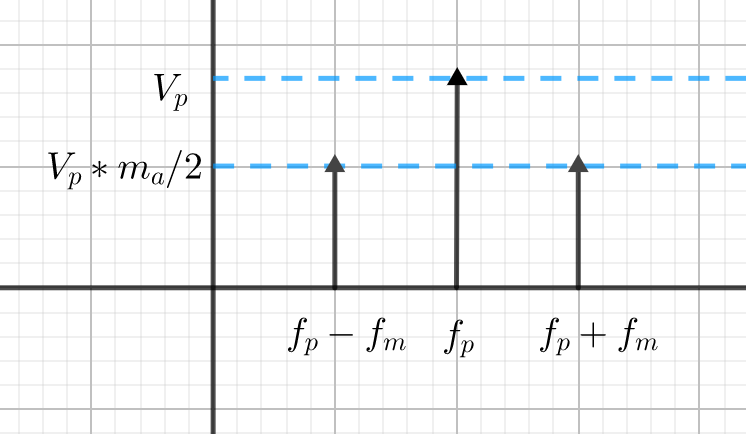
\includegraphics[width=\linewidth]{images/spettroAM.png}
  \caption{Spettro in frequenza di una modulazione AM}
  \label{fig:modAM}
\end{figure}

\section{Potenza della modulazione AM}
La potenza utilizzata dal segnale modulato è semplicemente la somma delle potenze delle sue 3 componenti. Come visto nel capitolo precedente, il segnale modulato è la somma pesata di 3 sinusoidi, rispettivamente alle frequenze $f_p - f_m$, $f_p$ e $f_p + f_m$. La potenza totale sarà quindi data da:
$$
P_{tot} = P_p + P_{bi} + P_{bs} 
$$
sapendo che con $bi$ si intende la banda inferiore e con $bs$ quella superiore. Ora, sapendo che la portante non contiene informazione e che le due bande laterali trasportano invece la stessa informazione, possiamo calcolare il rendimento $\eta$:
$$
\eta = \frac {P_{bi}}{P_{tot}}
$$
Cerchiamo ora di trovare una relazione tra i rendimento $\eta$ e l'indice di modulazione $m_a$. Sappiamo che data una resistenza generica $R$, la potenza di un segnale sinusoidale applicato a $R$ è 
$$
P = \frac{V_{eff}^2}{R}, \ \ V_{eff} = \frac{V_{picco}}{\sqrt{2}}
$$
Quindi le potenze delle nostre 3 componenti saranno:
$$
P_p = \frac{(\frac{V_p}{\sqrt{2}})^2}{R}
$$
$$
P_{bi} = \frac{(\frac{V_p * m_a}{2 * \sqrt{2}})^2}{R}
$$
$$
P_{bs} = \frac{(\frac{V_p * m_a}{2 * \sqrt{2}})^2}{R}
$$
le quali, sostituite nella:
$$
\eta = \frac{P_{bi}}{P_p + P_{bi} + P_{bs}}
$$
e applicando un po' di semplificazioni, daranno luogo ad una semplice soluzione:
$$
\eta = \frac{m_a^2}{2*m_a^2 + 4}
$$
Provando alcuni valori di $m_a$ come $0.2$, $0.5$ e $1.0$ si noterà che maggiore è l'indice di modulazione $m_a$, maggiore sarà il rendimento. Con il massimo $m_a$ possibile, cioè $1.0$, si ottiene un rendimento di $\frac{1}{6} = 16.6\%$.

Per incrementare ulteriormente il rendimento, sono necessari alcuni trucchetti::
\begin{itemize}
\item Trasmettere solo le bande laterali ed evitare di trasmettere la portante. Questa tecnica è chiamata modulazione AM DSB (double side band).
\item Trasmettere solo una delle due bande laterali, portando così il rendimento ad un teorico $100\%$. Questa tecnica è chiamata modulazione AM SSB (single side band).
\end{itemize}

\section{Demodulazione}
La demodulazione o rivelazione è un'operazione che consente di estrarre, da un segnale modulato in ampiezza, l'informazione in bassa frequenza (il nostro segnale originario $m(t)$).
Normalmente questa parte è realizzata tramite un circuito non-lineare, come un diodo seguito da un filtro passa-basso, i quali insieme sono in grado di ricostruire con buona approssimazione il segnale originario. \

Intuitivamente, il diodo si occupa di eliminare tutta la parte negativa del segnale modulato grazie alla sua proprietà di permettere il passaggio della corrente in un solo verso, mentre il filtro passa-basso (composto da una resistenza ed un condensatore) "riempie" gli spazi tra le oscillazioni ad alta frequenza. Questo grazie alla capacità del condensatore di immagazzinare cariche sulla cresta dell'onda sinusoidale e di rilasciarle subito dopo, per riempire il buco tra la cresta attuale e quella successiva.
\end{document}





